%%%%%%%%%%%%%%%%%%%%%%%%%%%%%%%%%%%%%%%%%
% Beamer Presentation
% LaTeX Template
% Version 1.0 (10/11/12)
%
% This template has been downloaded from:
% http://www.LaTeXTemplates.com
%
% License:
% CC BY-NC-SA 3.0 (http://creativecommons.org/licenses/by-nc-sa/3.0/)
%
%%%%%%%%%%%%%%%%%%%%%%%%%%%%%%%%%%%%%%%%%

%----------------------------------------------------------------------------------------
%	PACKAGES AND THEMES
%----------------------------------------------------------------------------------------

\documentclass{beamer}

\mode<presentation> {

% The Beamer class comes with a number of default slide themes
% which change the colors and layouts of slides. Below this is a list
% of all the themes, uncomment each in turn to see what they look like.


\usetheme{Madrid}

%\usecolortheme{albatross}
%\usecolortheme{beaver}
%\usecolortheme{beetle}
%\usecolortheme{crane}
%\usecolortheme{dolphin}
%\usecolortheme{dove}
%\usecolortheme{fly}
%\usecolortheme{lily}
%\usecolortheme{orchid}
%\usecolortheme{rose}
%\usecolortheme{seagull}
\usecolortheme{seahorse}
%\usecolortheme{whale}
%\usecolortheme{wolverine}


}

\usepackage{graphicx} % Allows including images
\usepackage{booktabs} % Allows the use of \toprule, \midrule and \bottomrule in tables
\usepackage{ngerman}
\usepackage[english]{babel}

\usepackage[utf8]{inputenc}
\usepackage{amsfonts}
\usepackage{amsmath}
\usepackage{amsthm}
\usepackage{amssymb}
\usepackage{subfigure}



\newcommand{\dX}{\mathcal{X}}
\newcommand{\dY}{\mathcal{Y}}
%----------------------------------------------------------------------------------------
%	TITLE PAGE
%----------------------------------------------------------------------------------------

\title[MIS Project]{OctoPocus} % The short title appears at the bottom of every slide, the full title is only on the title page

\author{Magdalena Keil and Jula McGibbon} % Your name
\institute[BUW] % Your institution as it will appear on the bottom of every slide, may be shorthand to save space
{
Bauhaus Universität Weimar  % Your institution for the title page
}
\date{\today} % Date, can be changed to a custom date

\begin{document}

\begin{frame}
\titlepage % Print the title page as the first slide
\end{frame}

\begin{frame}
\frametitle{Overview} % Table of contents slide, comment this block out to remove it
\tableofcontents % Throughout your presentation, if you choose to use \section{} and \subsection{} commands, these will automatically be printed on this slide as an overview of your presentation
\end{frame}

%------------------------------------------------
\section{Introduction to the original paper} 

\section{Own implementation}

\section{Live demo}

%----------------------------------------------------------------------------------------
%	PRESENTATION SLIDES
%----------------------------------------------------------------------------------------
%------------------------------------------------

\begin{frame}
\frametitle{Original Paper: Core Ideas}

\begin{figure}
\centering
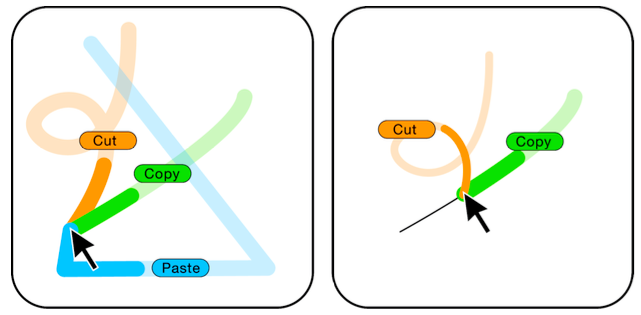
\includegraphics[width=0.54\textwidth]{ffpaths12.png}
	\caption{Left: Feedforward, Right: Feedforward and Feedback}
\end{figure}
\begin{itemize}
\item User can execute gestures dynamically in different directions
\pause
\item Each gesture evokes a different command, e.g. Paste, Copy, etc.
\pause
\item Learns to remember them after a few executions
\pause
\item Combination of an on-touch feedforward and feedback system
\pause
\item Less likely gesture paths become thinner or disappear entirely
\pause
\end{itemize}


\end{frame}
%------------------------------------------------

\begin{frame}
\frametitle{Feedforward mechanism}

\begin{figure}[H]
\centering
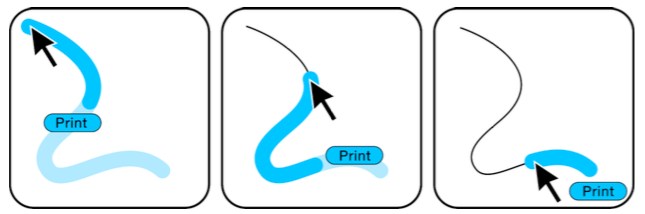
\includegraphics[width=0.65\textwidth]{ff.png}
\end{figure}

\begin{itemize}
\item Gives the user an impression of the gesture's shape and the related command
\pause
\item Each template gesture has a prefix starting at the cursor and marking a small part of the whole gesture in a deep color, the rest has the same but translucent color
\pause
\item The associated command is shown at the end of the prefix
\end{itemize}
\end{frame}

%------------------------------------------------

\begin{frame}
\frametitle{Feedback mechanism}

\begin{figure}[H]
\centering
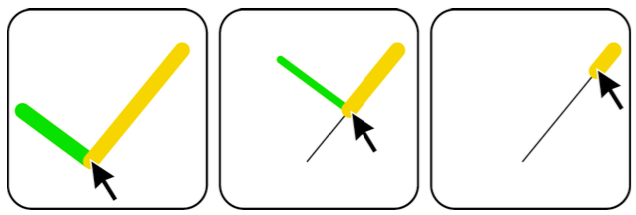
\includegraphics[width=0.65\textwidth]{fb.png}
\end{figure}

\begin{itemize}
\item Provides information about the recognition process after some action of the user 
\pause
\item Gesture recognition is accomplished by a classification algorithm using distance measures (Rubine's algorithm and Mahalanobis distance) 
\pause
\item The distances sum up to a consumable error rate until the input can no longer be recognized as a member of a given gesture class
\pause
\item The consumable error rate is also mapped onto the thickness of the gesture
%	\begin{itemize}
%	\item Initially all paths have the same thickness
%	\item The path being followed remains this thickness, if no errors have been made
%	\item Other paths become thinner as the error accumulates
%	\end{itemize}

\end{itemize}
\end{frame}

%------------------------------------------------

\begin{frame}
\frametitle{Novice or Expert?}

Novice version: 
\begin{itemize}
\item All paths are displayed by doing a long click \newline
\end{itemize}
\pause

Expert version: 
\begin{itemize}
\item No paths are displayed
\end{itemize}
\end{frame}


%------------------------------------------------


\begin{frame}
\frametitle{Own Implementation: Similarities to the original implementation}

\begin{itemize}
\item Gestures with different commands
\pause
\item OctoPocus resets itself if the user is returning back to the starting point
\pause
\item Feedforward: Prefix displays the next part to be drawn
\pause
\item Feedback: 
	\begin{itemize}
	\pause
	\item Already drawn path is shown in black 
	\pause
	\item Distance measure (Euclidean distance) as recognition tool, also mapped onto the path's 				  thickness
	\pause
	\item Likely paths have a fixed thickness
	\pause
	\item The less likely a path, the thinner it gets until it disappears
	\pause
	\end{itemize}
\item Novice and Expert mode
\end{itemize}
\end{frame}

%------------------------------------------------

\begin{frame}
\frametitle{Own Implementation: Differences to the original implementation}

\begin{itemize}
\item The starting point of the gesture is set at the touchdown of the finger (not variable after that)
\pause
\item We are working with touch and not with a cursor \newline $\Rightarrow$ Occlusion problems when paths are spread into all directions
\pause
\item One path is provided for the user to create his own gesture paths, replacing it with the old ones 
\end{itemize}
\end{frame}

%------------------------------------------------

\begin{frame}
\frametitle{Own Implementation: Important Issues}

\begin{itemize}
\item 1\$ recognizer:
	\begin{itemize}
	\item Was first considered for path recognition
	\item Complicated to work with for precise recognition
	\item Useful for Expert mode (?)\newline
	\end{itemize}
\pause
\item Finding the right thresholds:
	\begin{itemize}
	\item Paths can be drawn quite close to each other
	\item Solution: Doing error calculation only in the area close to the finger \newline
	\end{itemize}
\pause
\item Occlusion:
	\begin{itemize}
	\item All paths point into different directions by default
	\item Solution: Default paths can be modified by the \grqq New Path \grqq function, e.g. if the user is right-handed, he can draw all paths from the lower right to the left, upperleft and top direction
	\end{itemize}

\end{itemize}
\end{frame}

%------------------------------------------------

\begin{frame}
\frametitle{Live Demo}
\begin{figure}[H]
\centering
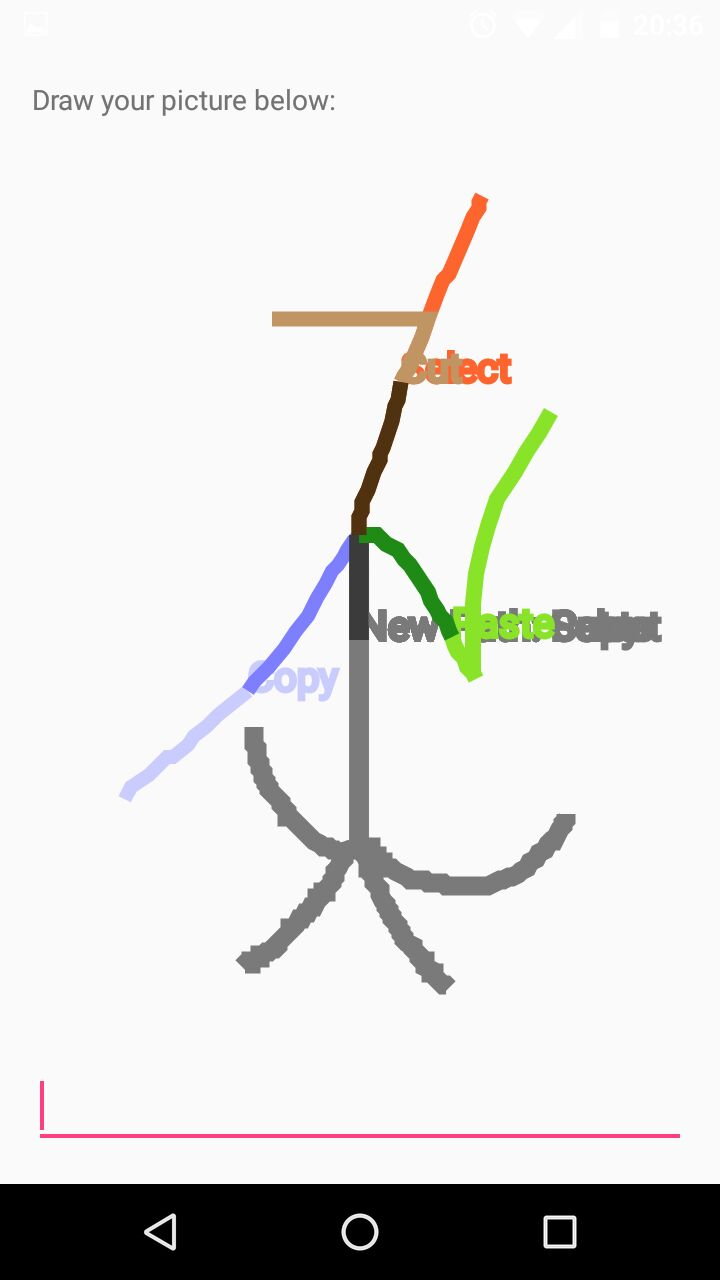
\includegraphics[width=0.35\textwidth]{myOctoPocus.png}
\end{figure}
\end{frame}

%----------------------------------------------------------------------------------------

\begin{frame}
\frametitle{References}
\footnotesize{
\begin{thebibliography}{99} % Beamer does not support BibTeX so references must be inserted manually as %below
\bibitem[Smith, 2012]{p1} Olivier Bau \& Wendy E. Mackay (2008)
\newblock Title of the publication
\newblock \emph{OctoPocus: A Dynamic Guide for Learning Gesture-Based Command Sets} 
\end{thebibliography}
}
\end{frame}

\end{document}